\documentclass{article}
\usepackage{graphicx}
\usepackage{amsmath}
\usepackage{cite}
\usepackage{color}
\usepackage{enumitem}
\usepackage{hyperref}
\usepackage{natbib}
\usepackage{tabularx}
\usepackage{natbib}
\usepackage{ragged2e}

\title{\textbf{La dis-informazione}}
\author{\texttt{Alessandro Meloni GEPID}}
\date{11/12/2023}

\begin{document}
\maketitle
    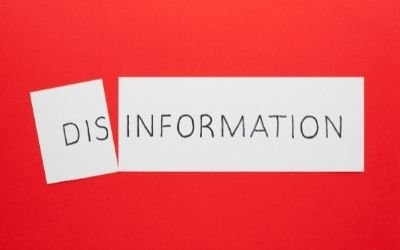
\includegraphics[width = 0.6\linewidth]{Immagini/disinformation.jpeg}
\centering \tableofcontents
\newpage \section{Introduzione}
\flushleft
\begin{justify}
    Questo articolo avrà prevalentemente la finalità di provare a mettere in chiaro cosa si intenda per disinformazione; e le varie sfaccettature che questo concetto può assumere.
    Faremo in modo di dare chiarezza in quanto la disinformazione ha di per sè una finalità negativa e di sviamento da ciò che è corretto, ma anche la sua forma non sempre risulta essere compresa agli occhi dei lettori.
    Innanzitutto faremo una piccola descrizione del concetto di disinformazione e le sue varie sfaccettature; successivamente analizzeremo una survey effettuata da parte dell'Unesco nel 2023, e, pubblicata dal \href{https://www.theguardian.com/technology/2023/nov/07/85-of-people-worry-about-online-disinformation-global-survey-finds}{The Guardian} come articolo nella loro pagina internet. Questo sarà seguito da un piccolo sondaggio fatto su un campione di X persone, provando a comprendere, almeno in Italia, quale possa essere la tendenza di percezione di questo concetto da parte della popolazione.
    Faremo e spiegheremo dei grafici risultanti dalla survey, così da comprendere quanto possano variare le percezioni sulla disinformazione sulla base di caratteristiche personali. 
    Seguirà successivamente una comparazione con alcuni dati relativi alla presenza oggettiva di fake news, così da capire se le percezioni delle persone, poi, coincidono con la frequenza oggettiva del fenomeno all'interno dei vari media.
    In conclusione, vedremo i risultati che ha dato questa ricerca, così da dare dei consigli su come riconoscere informazioni da dis-informazioni, con lo scopo di creare una maggiore consapevolezza e sicurezza nell'utente/lettore medio, evitando che questo fenomeno possa davvero portare al fine per cui la notizia viene diffusa.
    
\end{justify}
\begin{center}
\newpage \section{Il fenomeno della disinformazione}
\end{center}
\begin{justify}
    La disinformazione è quel fenomeno che viene studiato prevalentemente negli ambiti di scienze della comunicazione, ma che può espandersi a tanti rami.
    L'etimologia del termine risale al 1980, appunto perché venne per la prima volta utilizzato il termine russo \textit{dezinformatzija}, che si riferisce a "un'arma" che venne istituita dal KGB, e che consisteva semplicemente nel creare un ufficio ad hoc finalizzato alla diffusione e gestione della disinformazione, come attività di intelligence.\citep{DisWiki}\\
    Quindi dalla creazione dell'ufficio, iniziò a diffondersi questa terminologia, andando a colpire tutti gli stati mondiali, chi può e chi meno.
\end{justify}

\flushleft \subsection{Cos'è la disinformazione?}
\begin{justify}
    La disinformazione è un concetto molto ampio, e bisogna subito mettere in chiaro il fatto che non si riferisca esclusivamente a intenzioni malevoli, di fatto, è giusto, come definito dalla sociologa \texttt{Claire Wardle}, suddividere questo concetto in tre ramificazioni, comprendendo:
\begin{itemize}
    \item Disinformazione: la diffusione di notizie false con lo scopo specifico di trarre in inganno e sviare singoli soggetti, organizzazioni di persone o popolazioni intere: molte volte con finalità strettamente collegate ad ambito politico, finanziario ed interessi egoistici;
    \item Misinformazione: questo termine viene preso dall'inglese "misinformation" e indica un'informazione che di per sè è falsa, ma senza l'effettiva finalità di nuocere altrui soggetti da parte di colui o coloro che la diffondono. Certe volte è collegata alla diffusione di pezzi di informazione di un contenuto più ampio, senza sapere che esiste questo contenuto.
    \item Malinformazione: questo termine si distacca dalla normale definizione di "notizia falsa", però è opportuno ricomprenderla perchè ha come contenuto una notizia vera, ma che viene diffusa senza specificare il contesto, così da arrecare danno ad uno specifico soggetto o soggetti coinvolti nella notizia. \citep{wardle2018information}
\end{itemize}
\end{justify}

\newpage\flushleft \subsection{Analisi dati:}

\flushleft \subsection{L'impatto della disinformazione nella vita delle persone}

\centering
\newpage\section{Riflessioni e conclusioni}

\newpage\bibliography{Bibliografia}
\bibliographystyle{unsrtnat}
\end{document}